\AddToShipoutPictureBG*{
    \AtPageLowerLeft{
        
\includegraphics[width=\paperwidth,height=\paperheight]{chapters/chapter3.jpg}
    }
}

\decorate{默契}

\pagestyle{empty}

\Large
\begin{center}
    \vspace*{1.5cm}
    \color{white}
    {
    雁阵裁开天空的信封 \par \vspace*{0.4cm}
    北京的银杏数着光斑 \par   \vspace*{0.4cm}
    风翻阅落叶的日记 \par\vspace*{0.4cm}
    写下金色的注脚 \par\vspace*{0.4cm}
    风提着裙裾走过林间 \par\vspace*{0.4cm}
    枫叶在枝头酝酿绯红的诗篇 \par\vspace*{0.4cm}
    而我们在晨雾中 \par\vspace*{0.4cm}
    站成相望的桅杆 \par \vspace*{0.4cm}
    暮色浸透山峦时 \par \vspace*{0.4cm}
    柿子树点亮灯笼 \par \vspace*{0.4cm}
    我们走过的路正被落叶 \par \vspace*{0.4cm}
    装订成温暖的书脊
    }

    \vfill 
    \makefoot
\end{center}

\card{covers/cover8.jpg}{H}{希望你快乐}{Hope you are happy}

\setstyle{Hope you are happy}

\subtitle{天津之眼——摩天轮}

\large
\begin{spacing}{2}
    天津之眼，这座巨大的观景轮，就立在母亲河海河那温柔的臂弯里。它像一个来自未来的银色圆环，
    带着某种超现实的诗意，悬停在津门那片揉杂了哥特尖顶与玻璃幕墙的天际线上。
    它连接着望海楼教堂的古老钟声与对岸津湾广场的摩登光影，像一枚别在时间衣襟上的银色胸针，
    既见证着海河流淌百年的沧桑故事，也即将见证我们平凡而珍贵的相遇。

    白日的天津之眼，是冷峻的。那些精确交织的钢架在北方清澈的阳光下，反射出金属特有的锐利光泽，
    像一个严谨的数学公式，带着工业文明的理性与疏离。它静静地矗立在那里，如同一位来自异星的沉默观察者，
    冷静地俯瞰着桥上川流不息的车水马龙。然而，当暮色四合，华灯初上，它便完成了最动人的蜕变。
    周身亮起的蓝色光晕，瞬间柔化了所有坚硬的线条，让它化作这座城市最温柔、最深邃的瞳孔，
    在渐浓的夜色里，脉脉含情地注视着每一对从它脚下走过的有情人。

    我们是坐着公交车晃晃悠悠去的。晚高峰的车厢也并没有很拥挤，弥漫着疲惫与归心似箭的气息。
    我们混在其中，却像两个成功逃课的孩子，前后坐在公交车座椅上，怀揣着一种要去往秘密基地的、
    不足为外人道的兴奋。到站下车没多久，一个巨大的人形玩偶热情地扑上来，用毛茸茸的胳膊硬是将你搂在一起，
    “咔嚓”一声定格了一张合影。随即，那可爱的外壳下便伸出一只属于商人的、精明的手，索要陪拍摄费用。
    那一刻的尴尬与错愕，如今回想，却像一颗怪味豆，为那个夜晚增添了独特的滋味。所幸，我们像两个并肩作战的战友，
    在对方坚定的眼神里获得了勇气，最终从那场小小的商业围剿中成功“突围”。这个令人哭笑不得的插曲，非但没有扫兴，
    反而让我们的手在接下来的路上牵得更紧，仿佛共同守护了一个小小的、属于我们的秘密。

    脱身后，我们沿着河岸慢慢走。那巨大的光轮便在身侧缓缓移动，它不再是那个遥远的地标，而成了一个忠诚的伴侣，
    一个专程来护送我们夜行的、人间的月亮。晚风从河面上吹来，带着水汽的微凉，也捎来了远处街头艺人那把旧吉他弹唱的、
    若有若无的情歌。摩天轮的倒影跌落进墨色的海河里，被粼粼的水波揉碎，又顽强地一次次重新聚合，
    在水下构筑起另一个摇曳生姿的、梦境般的光轮。真实与虚幻，在此岸与彼岸间遥相呼应，仿佛一种隐喻——就像我们，
    本是独立的个体，却被一种不可言说的引力紧紧相连，共同构成了一个完整的圆。偶尔有装饰着彩灯的游船破开平静的水面，
    掀起的波浪将水中的光轮打散成万千跳跃的金色光点，它们闪烁、沉浮，又慢慢地、执着地重新聚拢，
    像极了生命中那些注定要相遇的缘分，无论经历怎样的波折，终会再次汇聚。

    仰起头，它像一个印在夜幕上的、发着光的巨大句读，为我们那一日的津门漫游，庄重地圈下了一个圆满的结尾。
    但我知道，这绝非故事的终点。正如摩天轮永恒的圆周运动，每一次的结束，都意味着新一轮循环的开始。
    在那个被红色灯带勾勒出的、温暖的光环下，我们所许下的，从来不是转瞬即逝的愿望，而是关于未来、关于永恒的，
    静默而郑重的承诺。

    % \begin{figure}[!htbp]
    %     \centering
    %     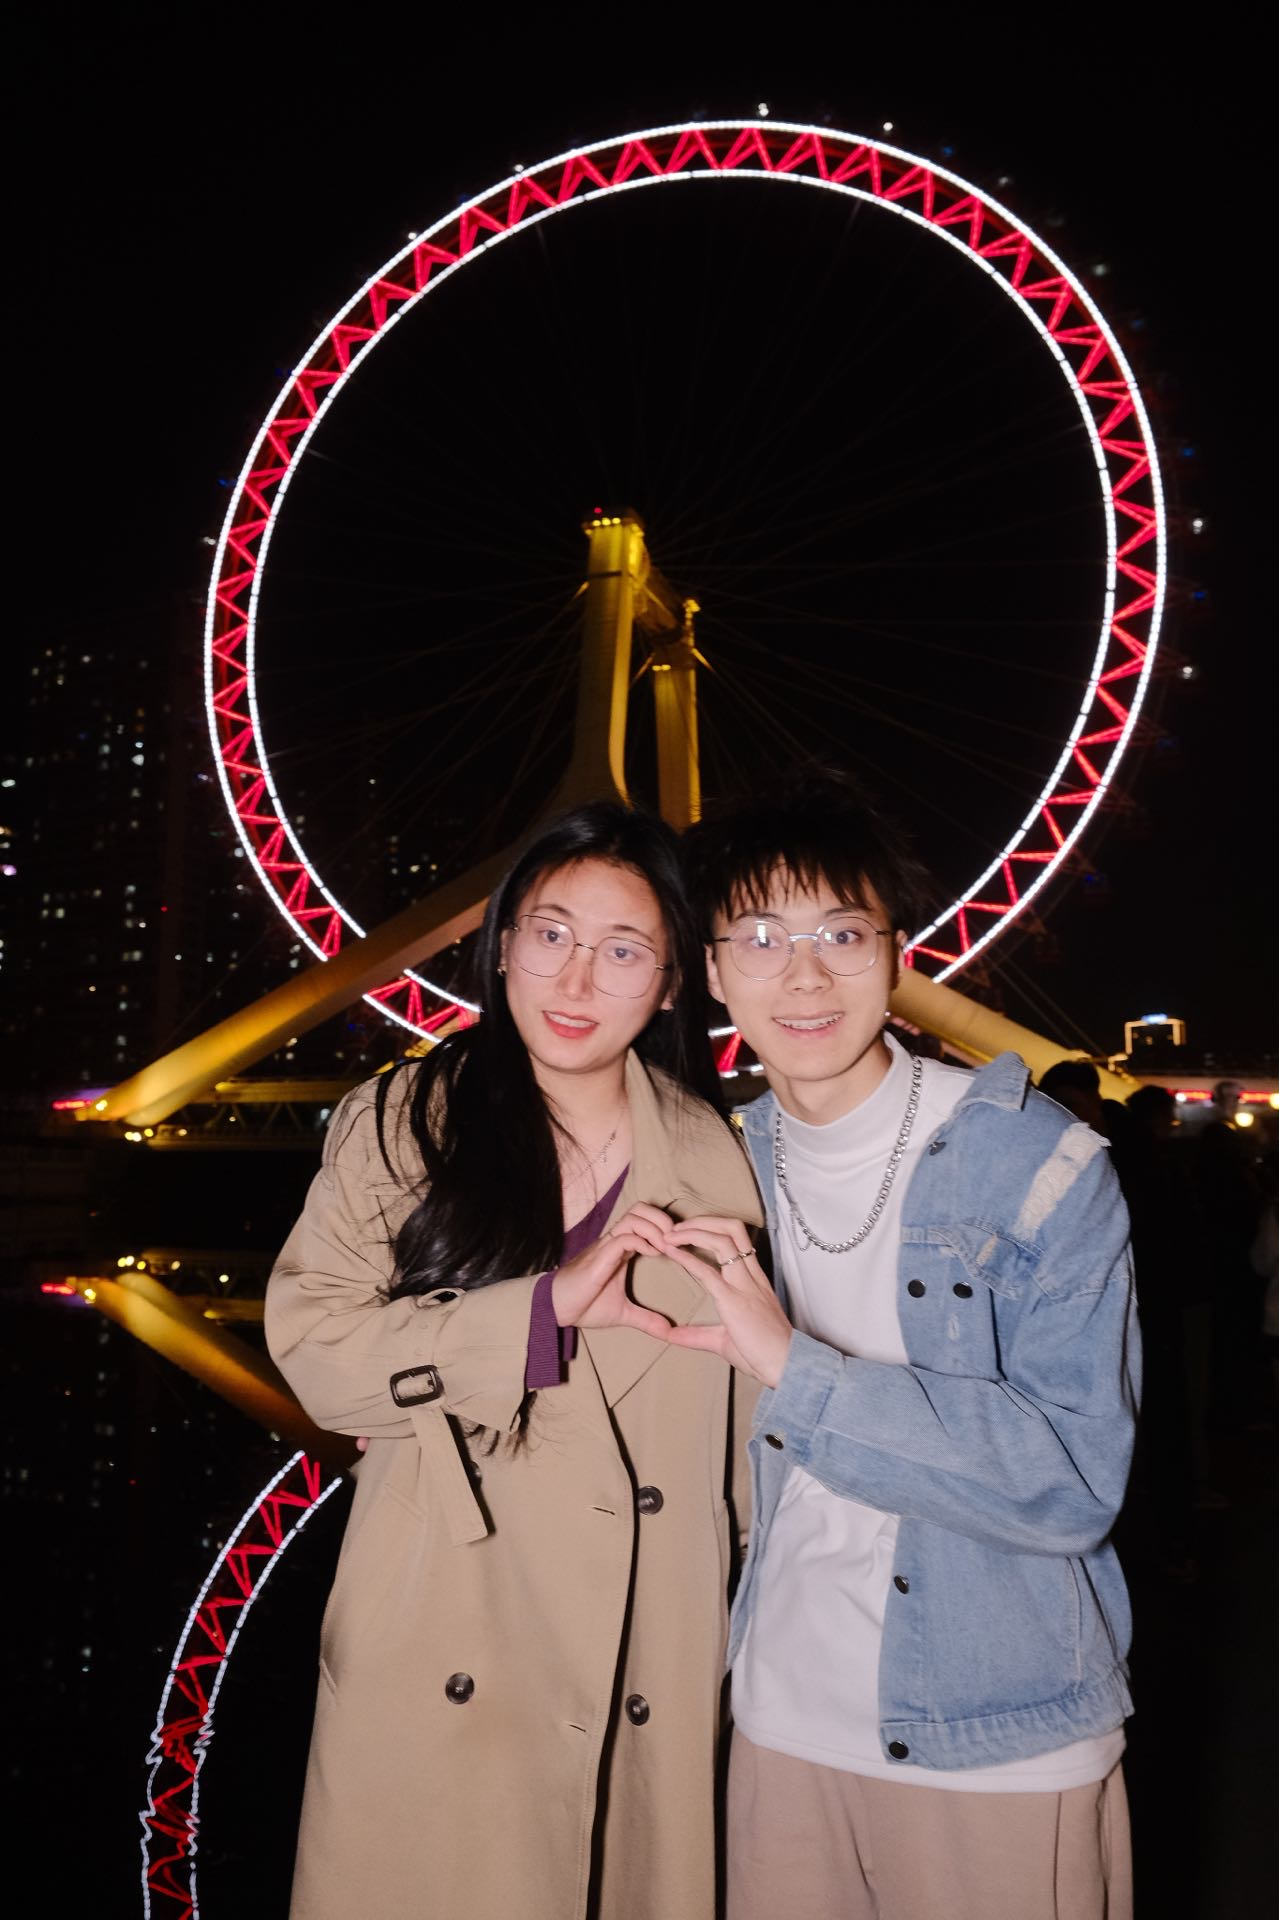
\includegraphics[width=0.6\textwidth]{figures/articles/02-1.jpg}
    %     \caption*{\small{2024年3月13日于天津之眼}}
    % \end{figure}

    \bottomtext{“与君初相识，犹如故人归。”}

\end{spacing}

\card{covers/cover9.jpg}{I}{我爱你}{I love you}

\setstyle{I love you}

\subtitle{钟久久——亦久久难忘}

\large
\begin{spacing}{2}
    它们不是被郑重地装在丝绒礼盒里递来的，没有聚光灯般的注视，也没有需要回应的誓言。
    只是在某个被阳光晒得慵懒的寻常午后，像两片被风吹来的银杏叶，自然而安静地，落在了我们摊开的掌心。

    那是两枚素净的银圈，光泽温吞，线条简洁，一如我们那时对爱的想象——不尚浮华，但求纯粹。

    没有单膝跪地的戏剧性场面，我只是轻轻托起你的手，将那枚微凉的银环缓缓推过你的指节。那一瞬间，
    金属的微凉在指根留下一个短暂的吻，旋即，便被我们身体里恒常的春天所接纳、同化，成为一种亲密的、皮肤的延伸，
    一种无言的体感温度。从此，它们便成了我们身体的一部分，参与并见证了我们所有的生活：它们在我们十指相扣时，
    于每一个稀松平常的日落之后，发出细微而清脆的碰撞声；它们也在我们紧紧相拥。

    如今，它们已经退出舞台了，那是时光与我们共同生活的证明。钟久久，亦，久久难忘。

    \bottomtext{“你在。我在。岁月长，我们在。”}
\end{spacing}

\card{covers/cover10.jpg}{J}{成为你想成为的样子}{Just be you}

\setstyle{Just be you}

\subtitle{津湾广场——津门灯火记事}

\large
\begin{spacing}{2}
    河水在脚下静静流淌，倒映着两岸截然不同的时空。对岸，解放北路上的老建筑群默然伫立，
    像一列身着晚礼服的旧时贵族，拱窗、石柱与雕花在暖黄灯带的勾勒下，愈发显得典雅而庄重。
    它们凝固了百年时光，每一扇窗后仿佛都藏着一个未完的故事。而我们这一侧，
    国金中心摩天的玻璃幕墙将整片夜空切割成几何的光块，冷白的灯光如星瀑般垂落，
    与河中颤动的倒影交相辉映。

    我们趴在河岸边的石栏上，肩并着肩，看了许久。春风裹挟着河水的微腥与城市的气息，从我们之间穿行而过。
    身后是解放桥上车水马龙流淌成的光河，引擎的低鸣与偶尔的汽笛是这座现代都市不变的背景音；身前，
    是那片沉默的、被灯火唤醒的“万国建筑博览苑”。而我们，就站在这道清晰的缝隙里——一边是凝固的历史，
    一边是流动的当下；一边是东方的土壤，一边是西洋的风貌。

    那一刻，我忽然觉得，我们看的不是风景，而是在共同阅读一本用灯火写就的、关于这座城市的厚重传记。
    每一盏在窗棂后亮起的温润的灯，都是一个被点亮的、充满烟火气的词语；每一座通体明亮、轮廓清晰的建筑，
    都是一段被完整照亮的、关于沉浮与新生的篇章。河面上，游船划开墨色的水，将那些金色的倒影揉碎又重组，
    像是书中翻动的页面。而我们共同的凝视与无言的沉默，便是为这本永恒的传记添上的、最新的一页，属于“我们”的注脚。

    夜渐深，灯火却愈发精神。我们离开河岸，走入那片光晕之中，身影也被镀上了一层暖融融的边。我们都在蠢蠢欲动，回头望去，津湾广场依旧静静地卧在海河畔，用它全部的明亮，对抗着整个夜晚的深沉。

    \begin{figure}[!htbp]
        \centering
        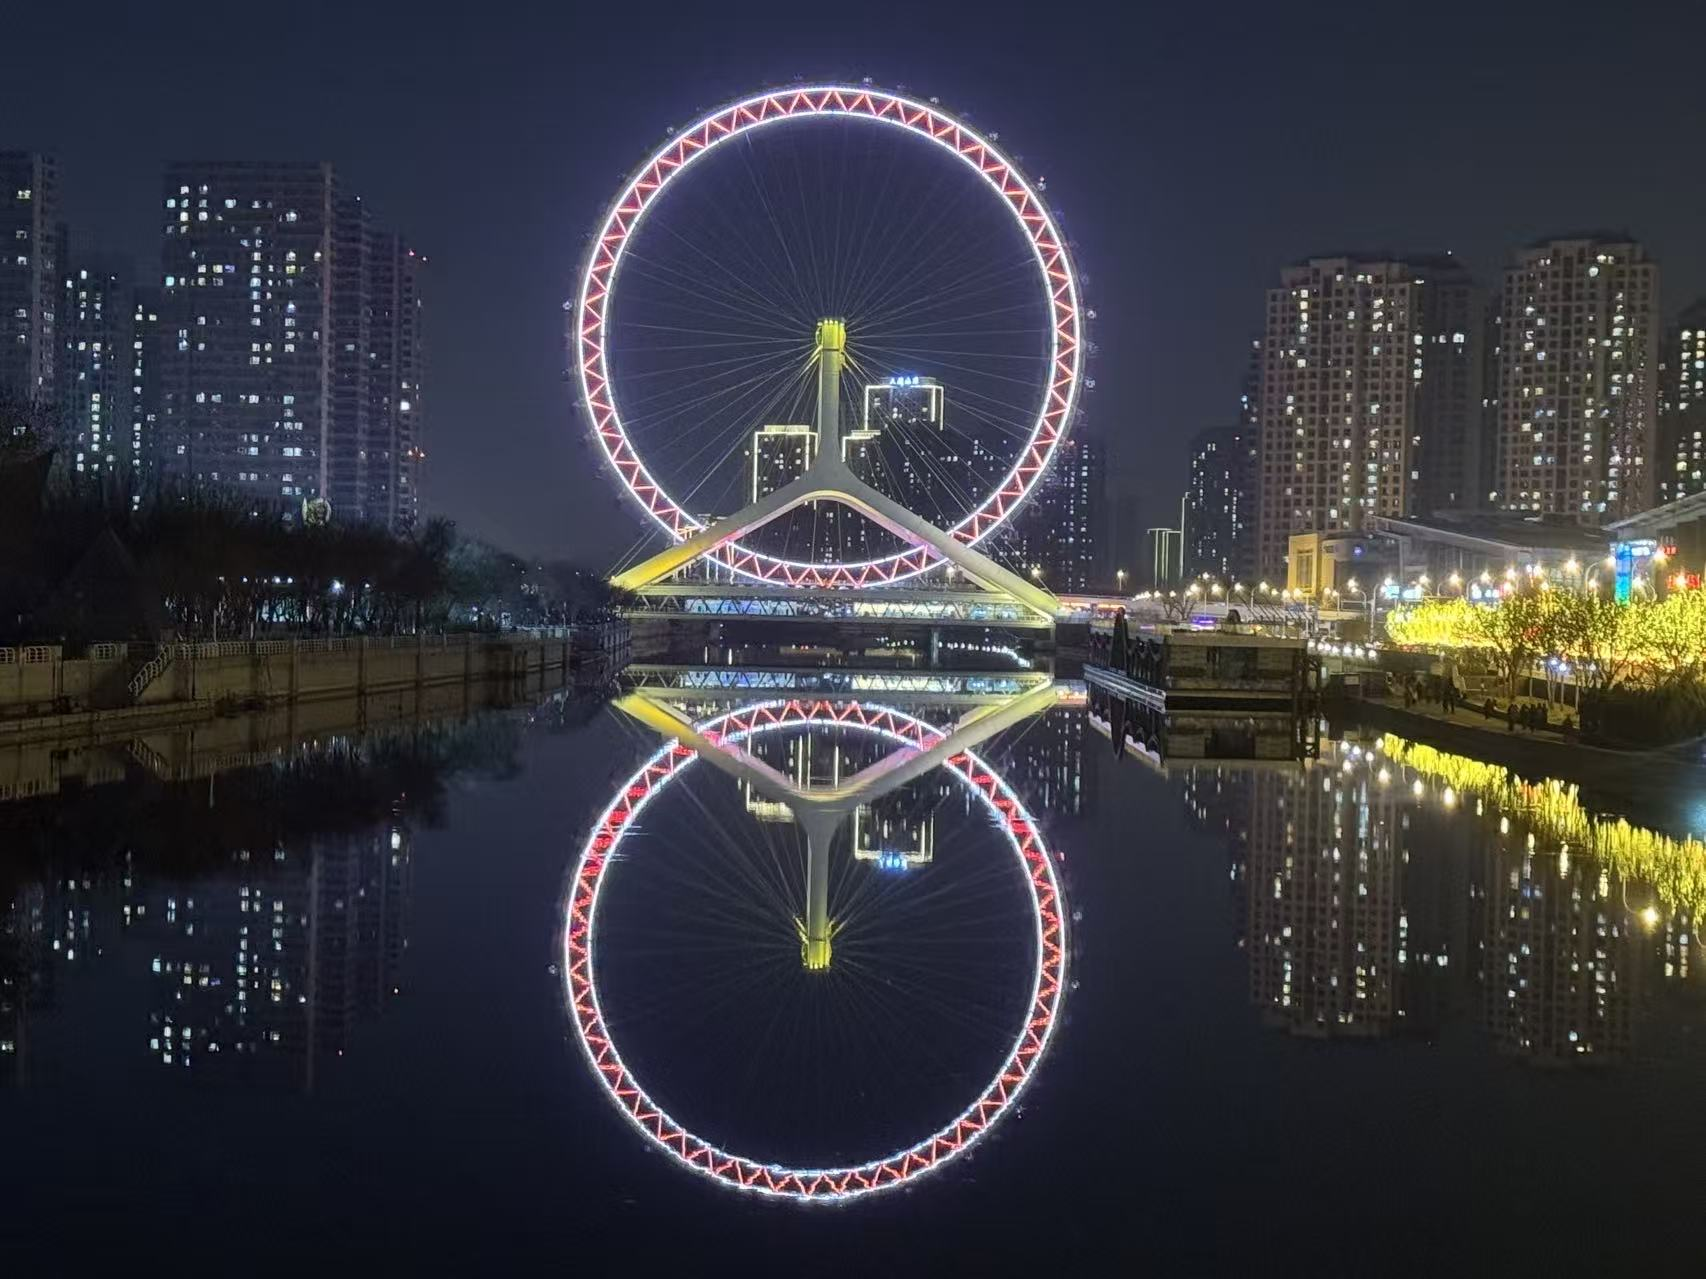
\includegraphics[width=0.8\textwidth]{figures/articles/02-2.jpg}
        \caption*{\small{2024年3月13日晚于天津之眼}}
    \end{figure}

    \bottomtext{“爱是唯一的真实，其余都是噪声”}
\end{spacing}

\card{covers/cover11.jpg}{K}{在你醒来时吻你}{Kiss you when you wake}

\setstyle{Kiss you when you wake}

\subtitle{天津日出日落——潮汐与光的协奏曲}

\large
\begin{spacing}{2}
    在滨海新区的那个黄昏与翌日清晨，我们听了一场由潮汐与光演奏的协奏曲。
    
    \begin{figure}[!htbp]
        \centering
        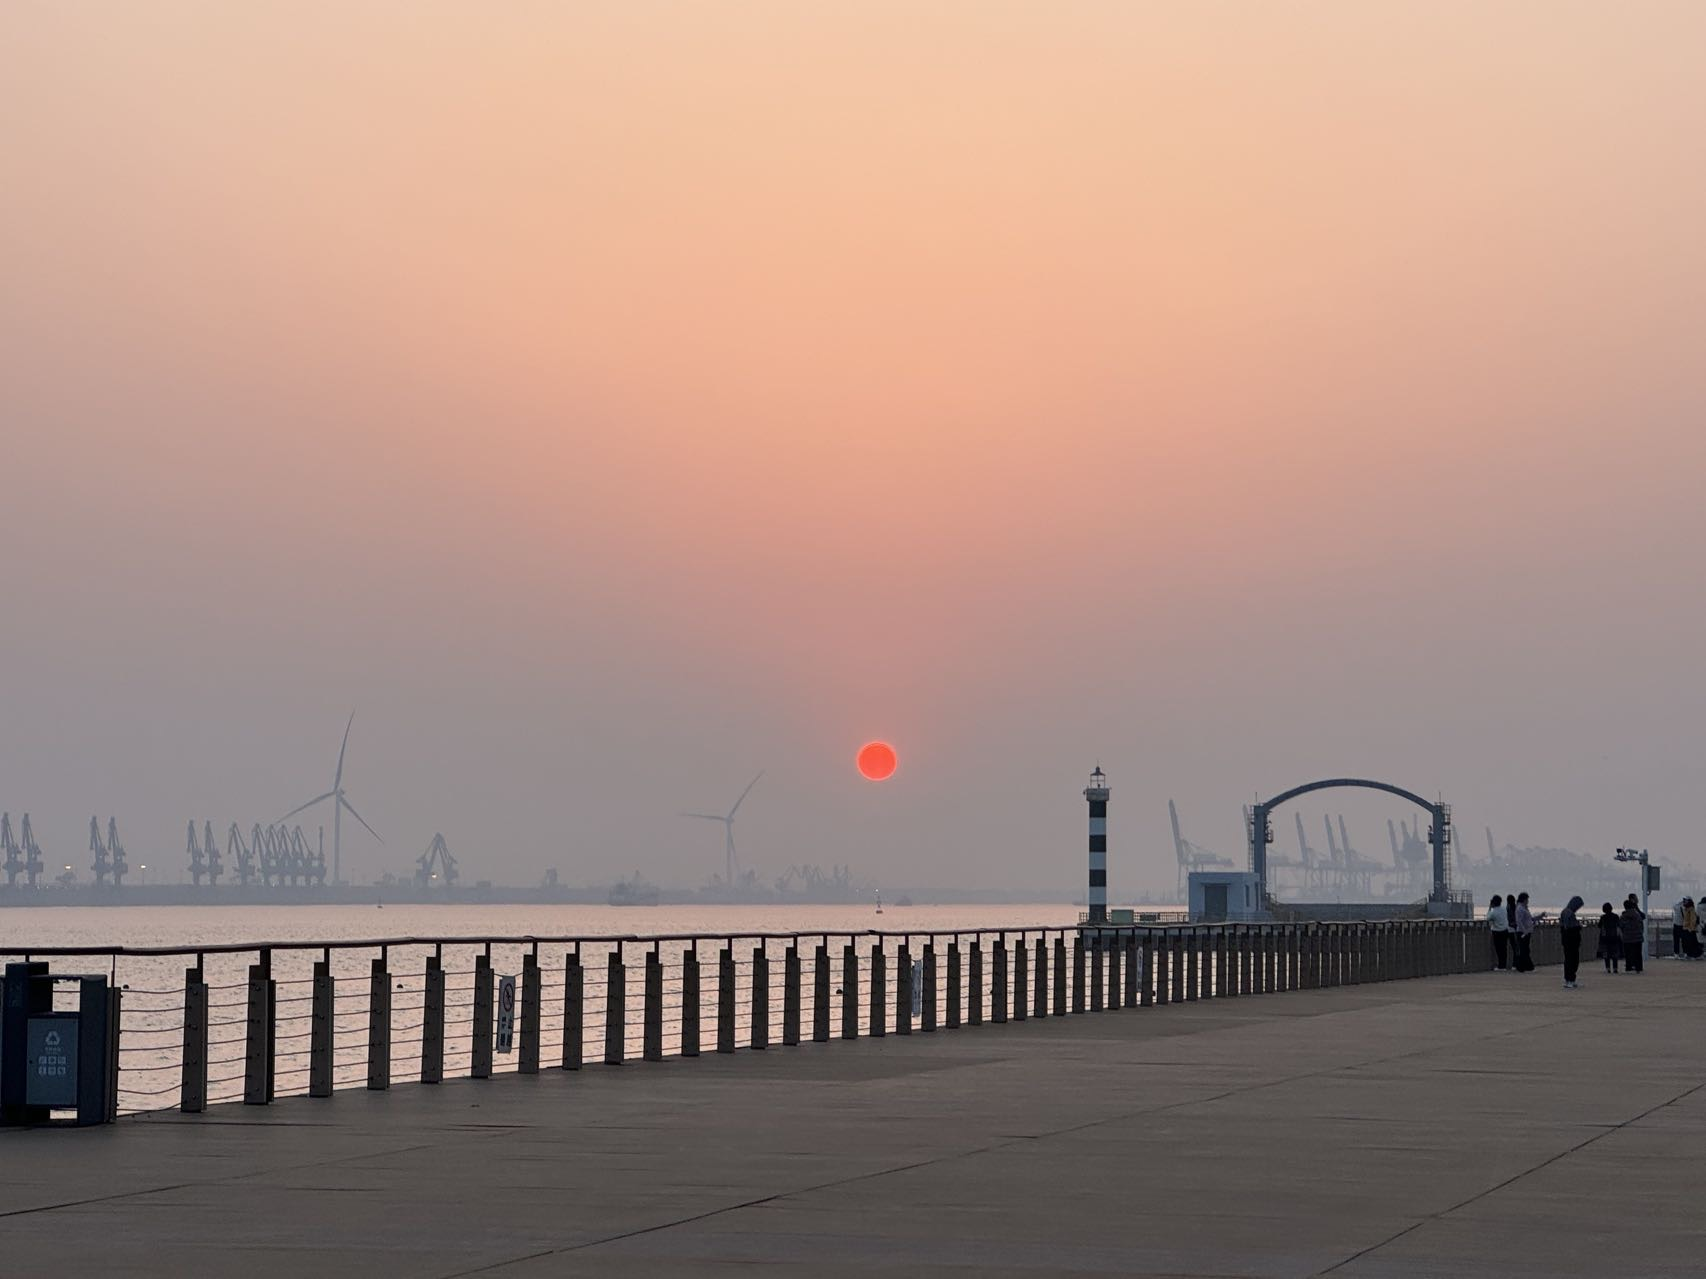
\includegraphics[width=0.6\textwidth]{figures/articles/02-3.jpg}
        \caption*{\small{2024年3月14日于东疆建设开发纪念公园}}
    \end{figure}

    傍晚时分，我们站在防波堤上。海风带着咸涩的气息，比市区里猛烈许多，吹得你的裙摆沙沙作响，像一面不肯投降的旗帜。太阳，那颗燃烧了一日的火球，正失去它咄咄的锋芒，变得像一颗温润的、巨大的咸蛋黄，缓缓向着海平面那条笔直的线沉降。


    那一刻，光不再是照耀，而是流淌。它把自己融化在波涛里，整片渤海于是变成一锅滚沸的金色熔岩。海浪不知疲倦地涌向堤岸，那哗啦哗啦的声响，浑厚而低沉，是大提琴的弓弦匀速拉过漫长的海岸线。每一道浪头的破碎，都溅起无数细碎的金芒，那是跳跃的、清脆的琶音。

    我们看着那轮落日被海水一寸寸吞没，像一场庄严的献祭。直到最后一线金光被墨蓝的海水抿去，世界并未立刻陷入黑暗，而是沉浸在一片由暖紫、玫红与橘色交织的、漫长的霞光里。潮声在暮色中显得愈发清晰，仿佛在为光明的退场奏响安魂曲。

    \begin{figure}[!htbp]
        \centering
        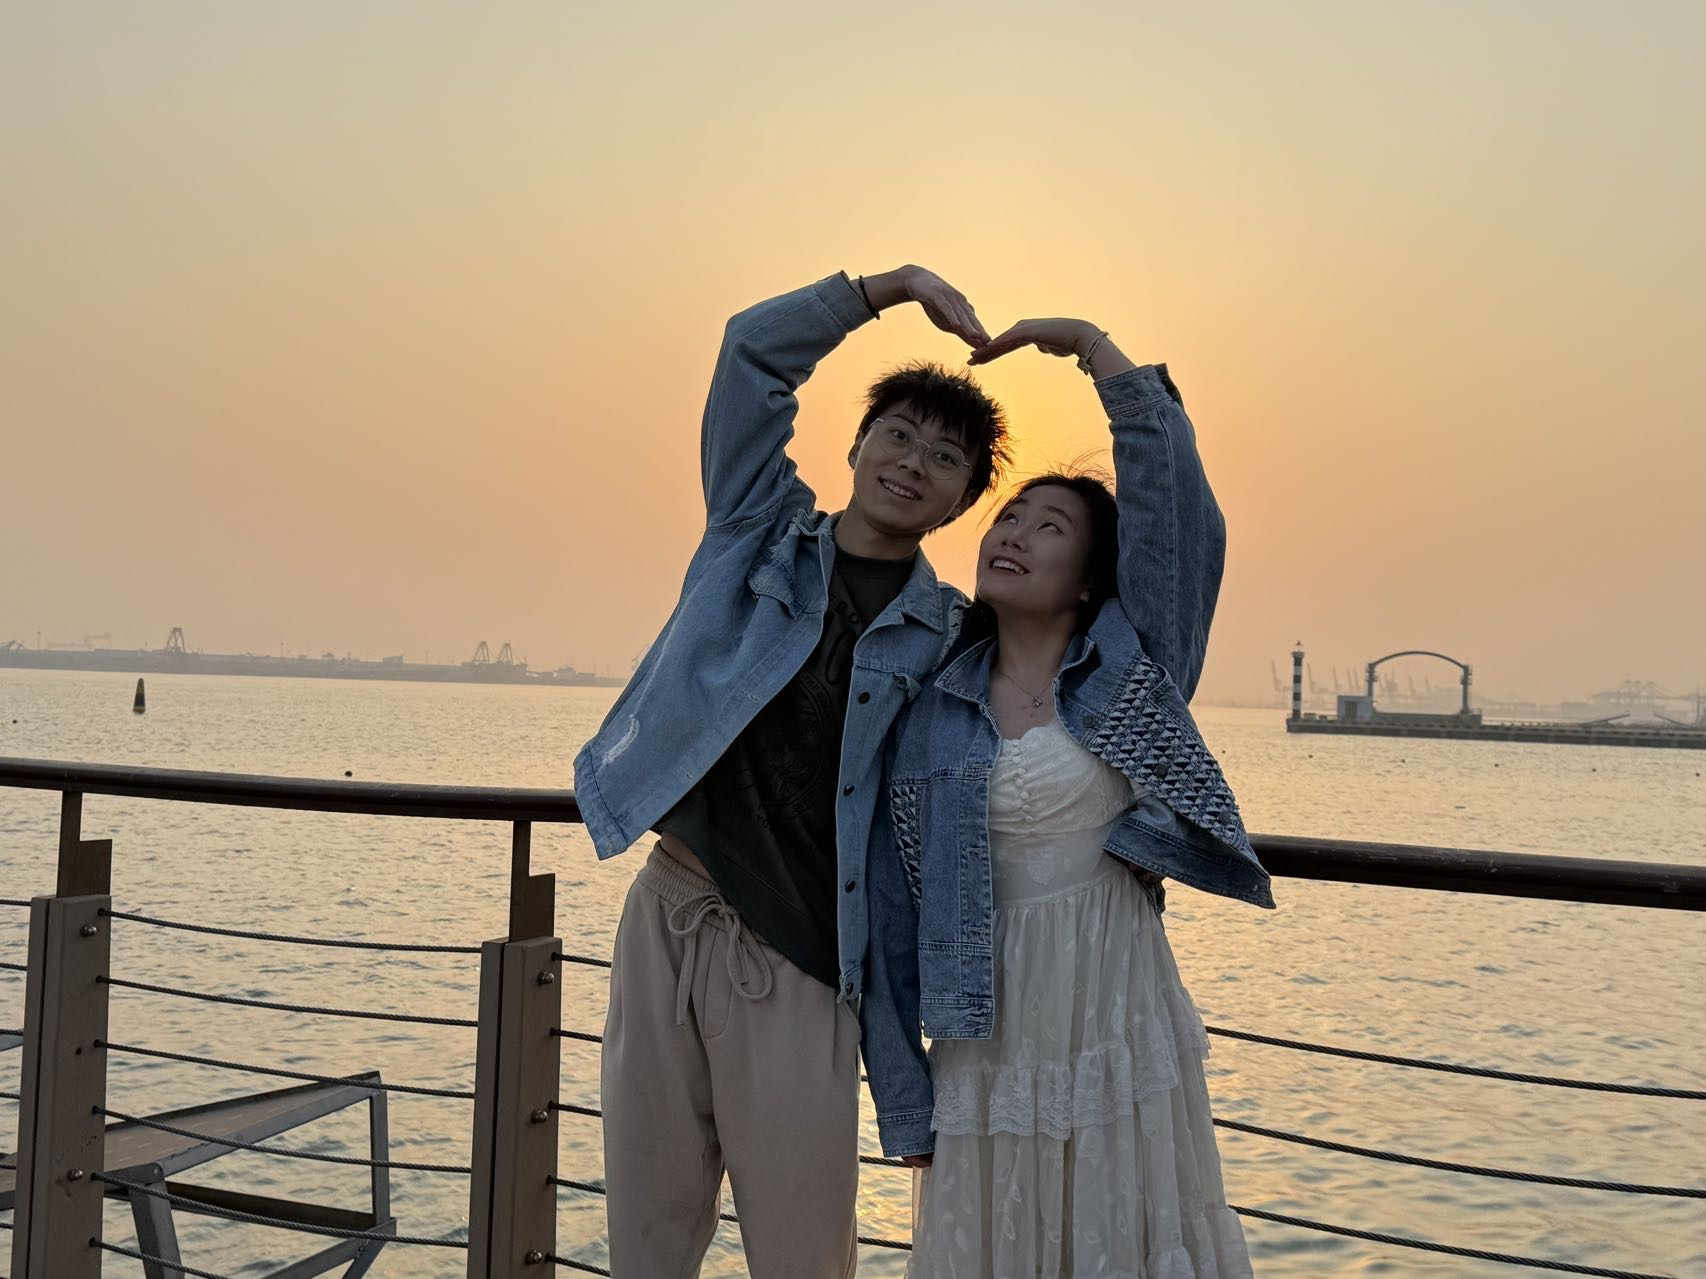
\includegraphics[width=0.8\textwidth]{figures/articles/02-4.jpg}
        \caption*{\small{2024年3月14日于东疆建设开发纪念公园}}
    \end{figure}

    日出与日落，本是同一枚太阳的轨迹。亲眼所见的、充满仪式感的诞生，其能量与光芒，早已蕴藏在我们共同经历的、那场盛大落幕之中。那日落时积蓄的所有温暖与辉煌，仿佛都化为了此刻照亮你脸庞的、温柔的光线。

    潮汐依旧，日升月落，是天地间永恒不变的循环律动。而我们，在这伟大的协奏曲里，我们都是追逐第一缕光的虔诚信徒，是两个在旋律中偶然相遇的音符，因彼此的陪伴，而找到了属于自己的、微小却坚定的和声。
    
    \begin{figure}[!htbp]
        \centering
        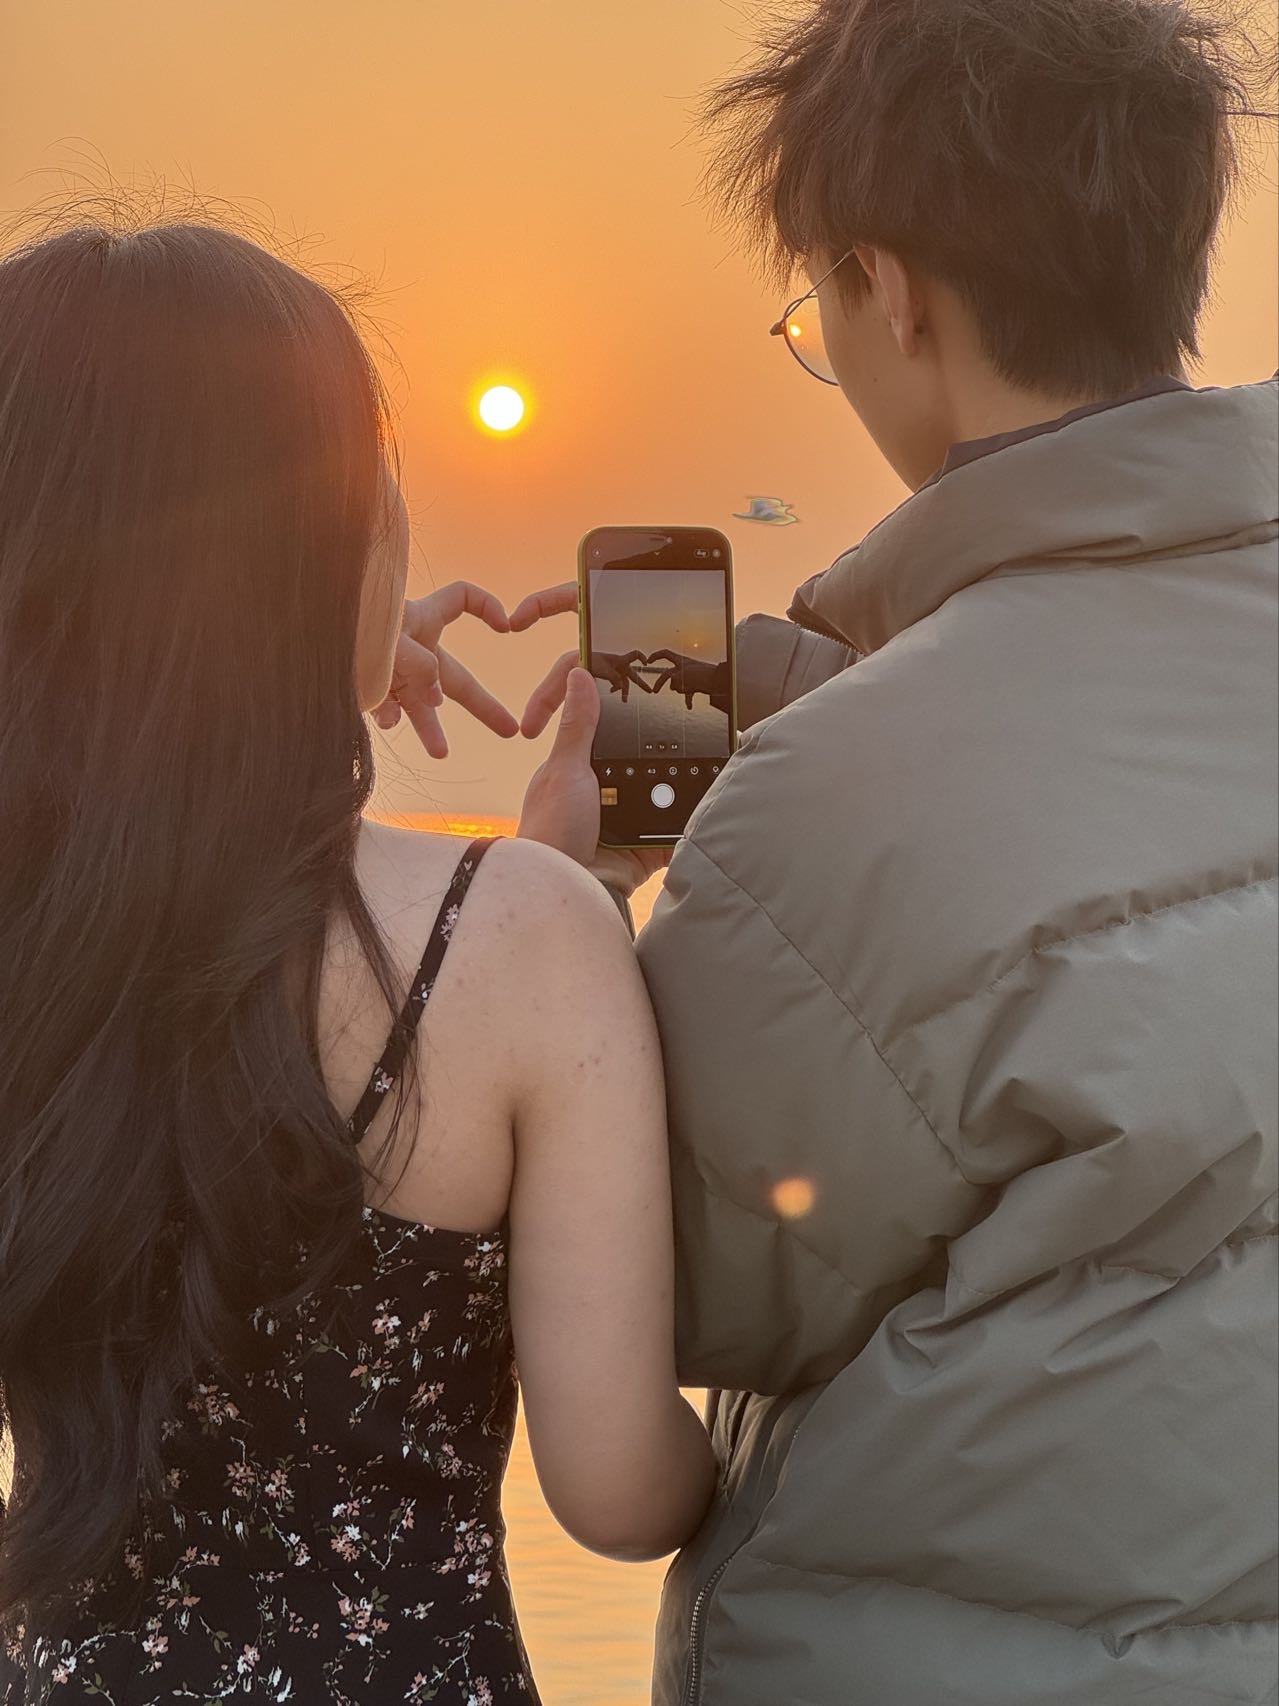
\includegraphics[width=0.4\textwidth]{figures/articles/02-5.jpg}
        \caption*{\small{2024年3月15日于东疆亲海公园}}
    \end{figure}

    在这场日出日落之后，似乎所有的日出日落我都并不感兴趣。无论是晨曦初升的金光，还是晚霞铺满的天际，都不再让我心动。唯有那一次——与你一同静坐在天与海交汇的地方，看第一缕光穿透云层，看最后一抹红隐入地平线。那一刻的风、那一刻的光、那一刻你的笑容，都成了我记忆中最柔软的风景。此后所有的日出日落，都成了那一次的回响。
    
    也是在这场日出日落之后，我才明白，原来风景之所以动人，是因为那时你在我身旁。没有你的晨曦显得冷淡，没有你的晚霞也失了色彩。世间的光影轮回千百次，但唯独那一次，我看见了你——于是天地都温柔了。
    
    \begin{figure}[!htbp]
        \centering
        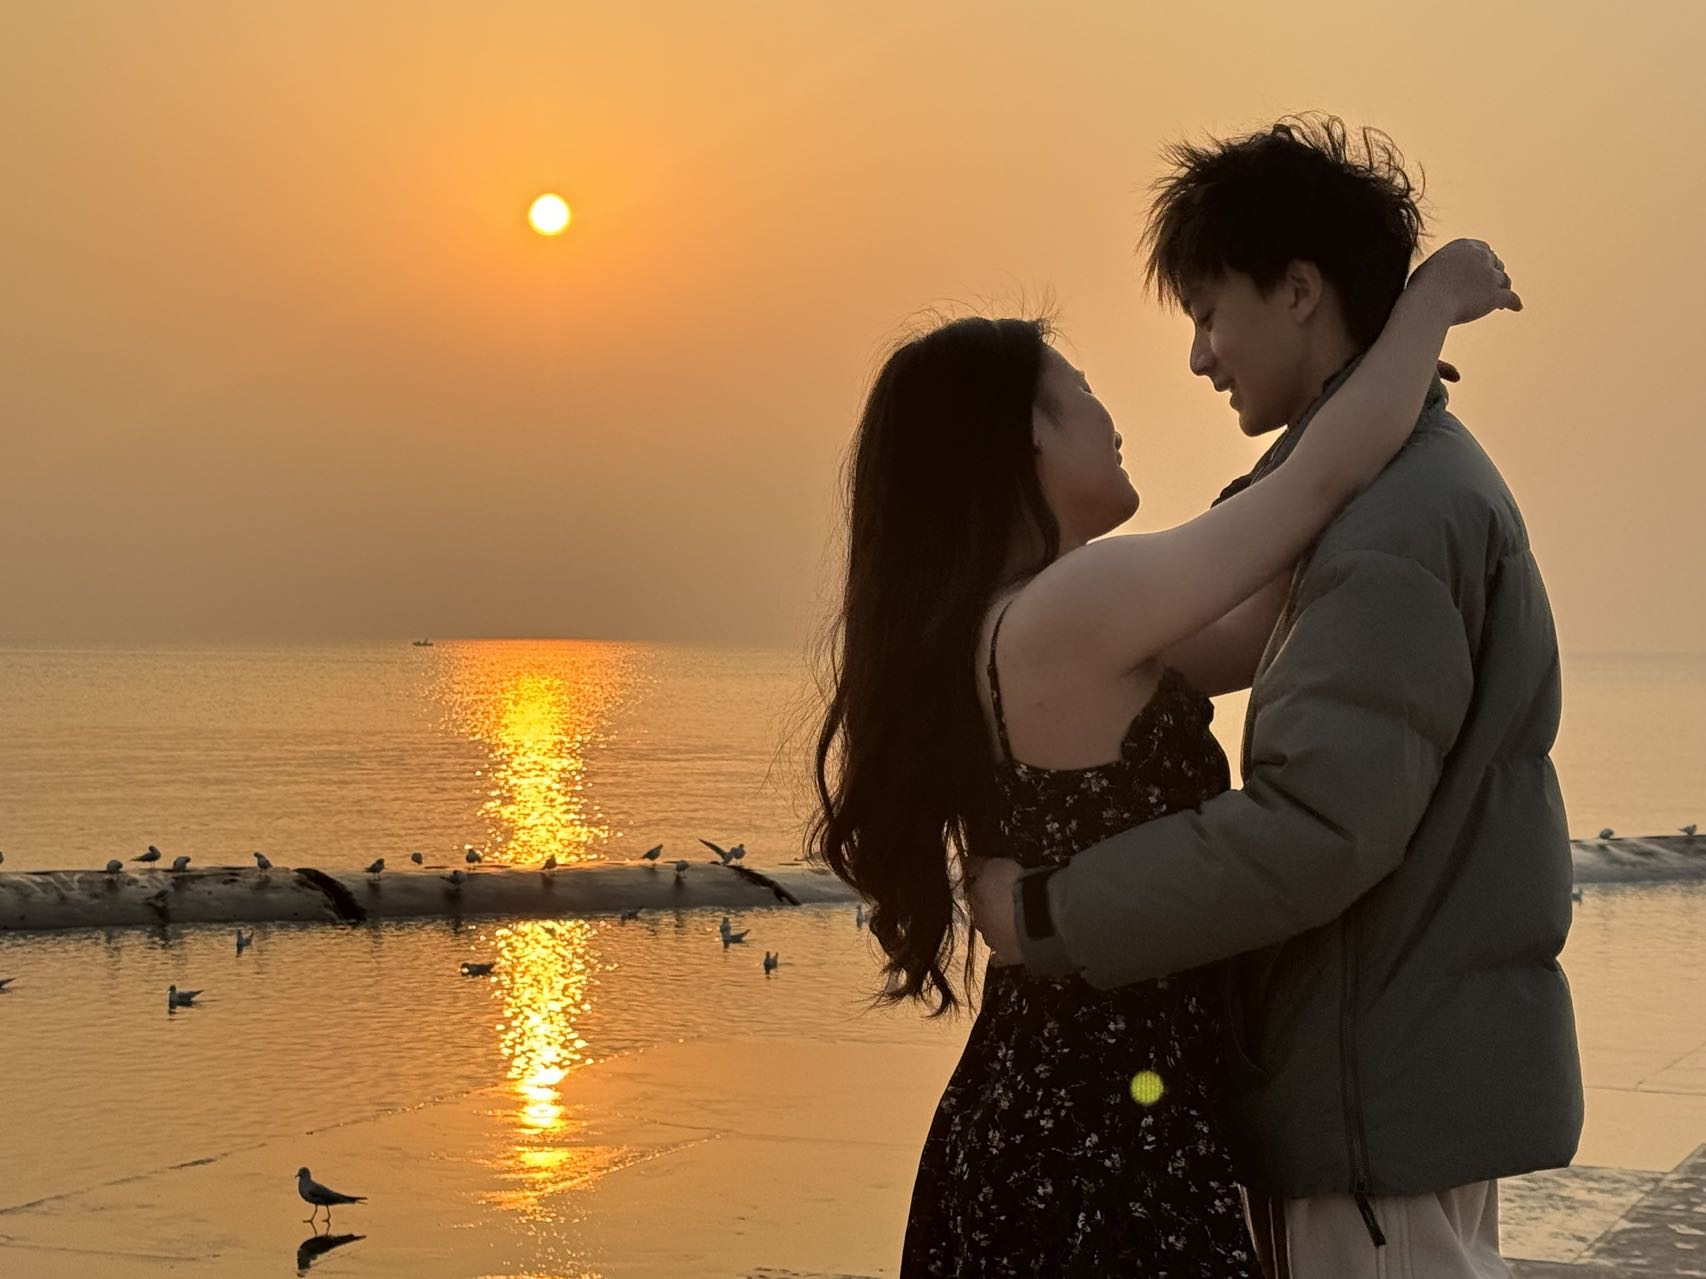
\includegraphics[width=0.8\textwidth]{figures/articles/02-6.jpg}
        \caption*{\small{2024年3月15日于东疆亲海公园}}
    \end{figure}

    \bottomtext{“山河远阔，人间烟火，无一是你，无一不是你”}
\end{spacing}

\card{covers/cover12.jpg}{L}{学会懂你}{Learn to know you}

\setstyle{Learn to know you}

\subtitle{海洋博物馆——蔚蓝百科序章}

\large
\begin{spacing}{2}
    滨海的风裹挟着微咸的湿气，像一块清凉的薄纱，轻轻拂过发烫的脸颊。那天我的身体提出抗议，但还是跟在你身后，
    缓缓驶入了那座名为“天津海洋博物馆”的蔚蓝殿堂。

    记忆从那一刻起，便自动褪去了具体的形状与色彩。如今回想，那日的展厅仿佛一个巨大而静谧的水族箱，
    我们漫步其中。我记不清那些展品的确切模样，只记得一片朦胧的、流动的蓝。我的感官变得迟钝，
    世界仿佛隔着一层毛玻璃，唯有你的身影是清晰的——你时而回头确认我的状态，时而为我隔开拥挤的人潮。
    那份无微不至的关心，是这片蓝色迷宫中唯一稳定的坐标，是照亮我昏沉世界的一束柔光。

    离去时，我倚在门廊回望。整座建筑的轮廓在暮色中渐渐模糊，融成一片深不见底的蓝。
    有些记忆缓缓地、缓缓地沉入这片记忆的水底，化作一场无声的、流动的梦。

    \bottomtext{“有些浪花不为靠岸而生，它们只是想看一眼光。”}
\end{spacing}

\card{covers/cover13.jpg}{M}{让我成为你生活的一部分}{Make me yours}

\setstyle{Make me yours}

\subtitle{五大道——海棠花荫记事}

\large
\begin{spacing}{2}

    春日的午后，阳光像被筛过一般，透过海棠花初绽的枝叶，在五大道的青石板路上投下细碎而晃动的光斑。
    我们手里各拿着一瓶瓷瓶老酸奶，那圆润的瓶身还沁着微微的凉意，像握着一小块尚未融化的春天。
    随意找了片无人的绿地坐下，草叶的清香混着酸奶醇厚而温柔的甜，便轻轻地弥漫在周围的空气里，
    成为一种私密的、只属于此刻的气息。

    风是慢的，带着些许历史沉淀下来的温润，从那一栋栋老洋房的红砖瓦顶、从雕花的石柱与紧闭的百叶窗间悄然掠过。
    它们静默地排列着，像一列矜持的旧时绅士，每一扇窗后都藏着一个沉睡的梦，每一片砖瓦都在低声讲述着泛黄的故事。
    而我们，误入此间的两个现代人，则像两页被风偶然吹开的日记，有幸在此刻，静静地融入这幅由岁月亲手绘制的、流动的画卷。

    我们就这样静静地坐着，一小口一小口地啜饮着手中的酸奶，看偶尔走过的游客，他们的脚步轻快，谈笑风生，
    却丝毫不惊扰我们这一隅被施了魔法的惬意。远处似乎有马车的铃铛声传来，清脆而遥远，更衬出此地的安宁。
    那一刻我忽然觉得，哪怕时间就此停顿，也好像无关紧要了——因为这整个下午的温柔，本身就已是我们共同记下的、
    一个完整而温暖的片段。它无需被刻意回忆，因为它已然成为我们生命质地的一部分。
    
    \begin{figure}[!htbp]
        \centering
        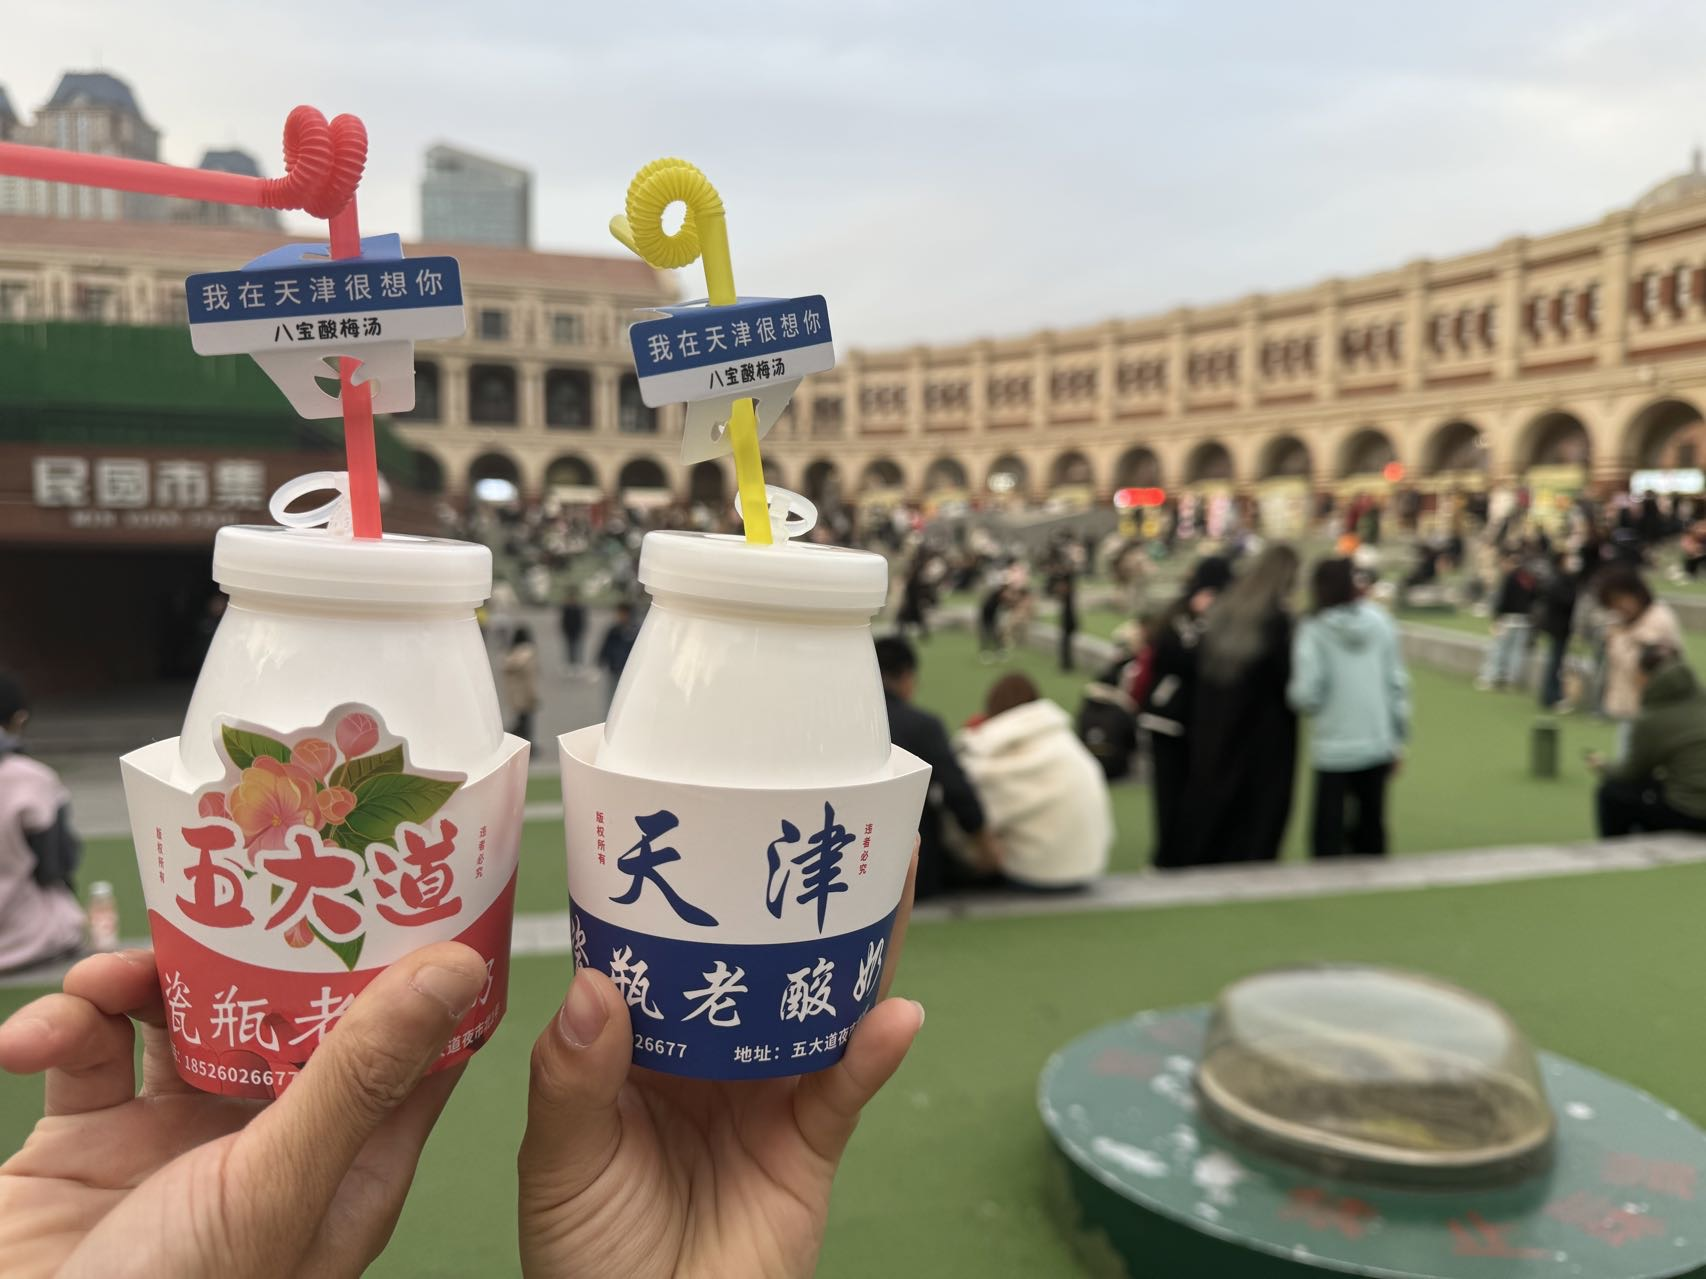
\includegraphics[width=0.8\textwidth]{figures/articles/02-7.jpg}
        \caption*{\small{2024年3月16日于天津五大道文化旅游区}}
    \end{figure}

    \bottomtext{“有些时光不为回忆而生，它只是悄悄停在你我之间。”}

\end{spacing}

\card{covers/cover14.jpg}{N}{永远不让你哭}{Never make you cry}

\setstyle{Never make you cry}

\subtitle{八一广场——洪都坐标}

\large
\begin{spacing}{2}
    我们随着人潮，匆匆穿过八一广场那片开阔而喧闹的热浪。脚步被四面八方涌来的声音推着向前——导游的喇叭声、
    孩子的嬉笑声、快门清脆的咔嚓声，交织成一首属于城市的行进曲。那是我与这座英雄城的初遇，
    带着初来者的新奇与张望；而你已是故地重游，眉眼间是熟稔的平静，却依旧耐心地陪着我，
    将我好奇的目光一一指认、解说。

    午后的阳光慷慨得有些刺眼，将纪念塔与飘扬的旗帜淬炼出耀眼的轮廓，在炽热的空气里微微晃动。
    光影在历史的浮雕上急速流转，我们像两个被时间驱赶的读者，只能快速地浏览这宏伟篇章的每一个角落，
    来不及细品，便已被推往下一页。
    
    当感官被庞杂的信息填满，饥饿感终于后知后觉地涌上。我们逃离广场的喧嚣，随意钻进附近商场里一家冒着热气的小店。
    又是牛蛙——坐下时我们相视一笑，这已经数不清是第几次共同投向这辛辣而肥美的慰藉了。店里人声鼎沸，
    油锅爆炒的滋滋声与香料浓烈的气味交织，构成一种极具烟火气的包围。我们在这片嘈杂中坐下，
    仿佛两只终于找到临时泊岸的小舟。

    那一餐吃得没有什么仪式感，甚至有些狼吞虎咽的仓促。但在辣椒与花椒带来的灼热感中，在彼此被热气熏得发红的脸上，
    一种奇异的安宁却悄然降临。它仿佛在告诉我们：旅途难免奔波，时光总是匆促，但真正珍贵的，
    正是我们善于在这些短暂的停顿里，偷得一份属于彼此的、滚烫的当下。
    
    \begin{figure}[!htbp]
        \centering
        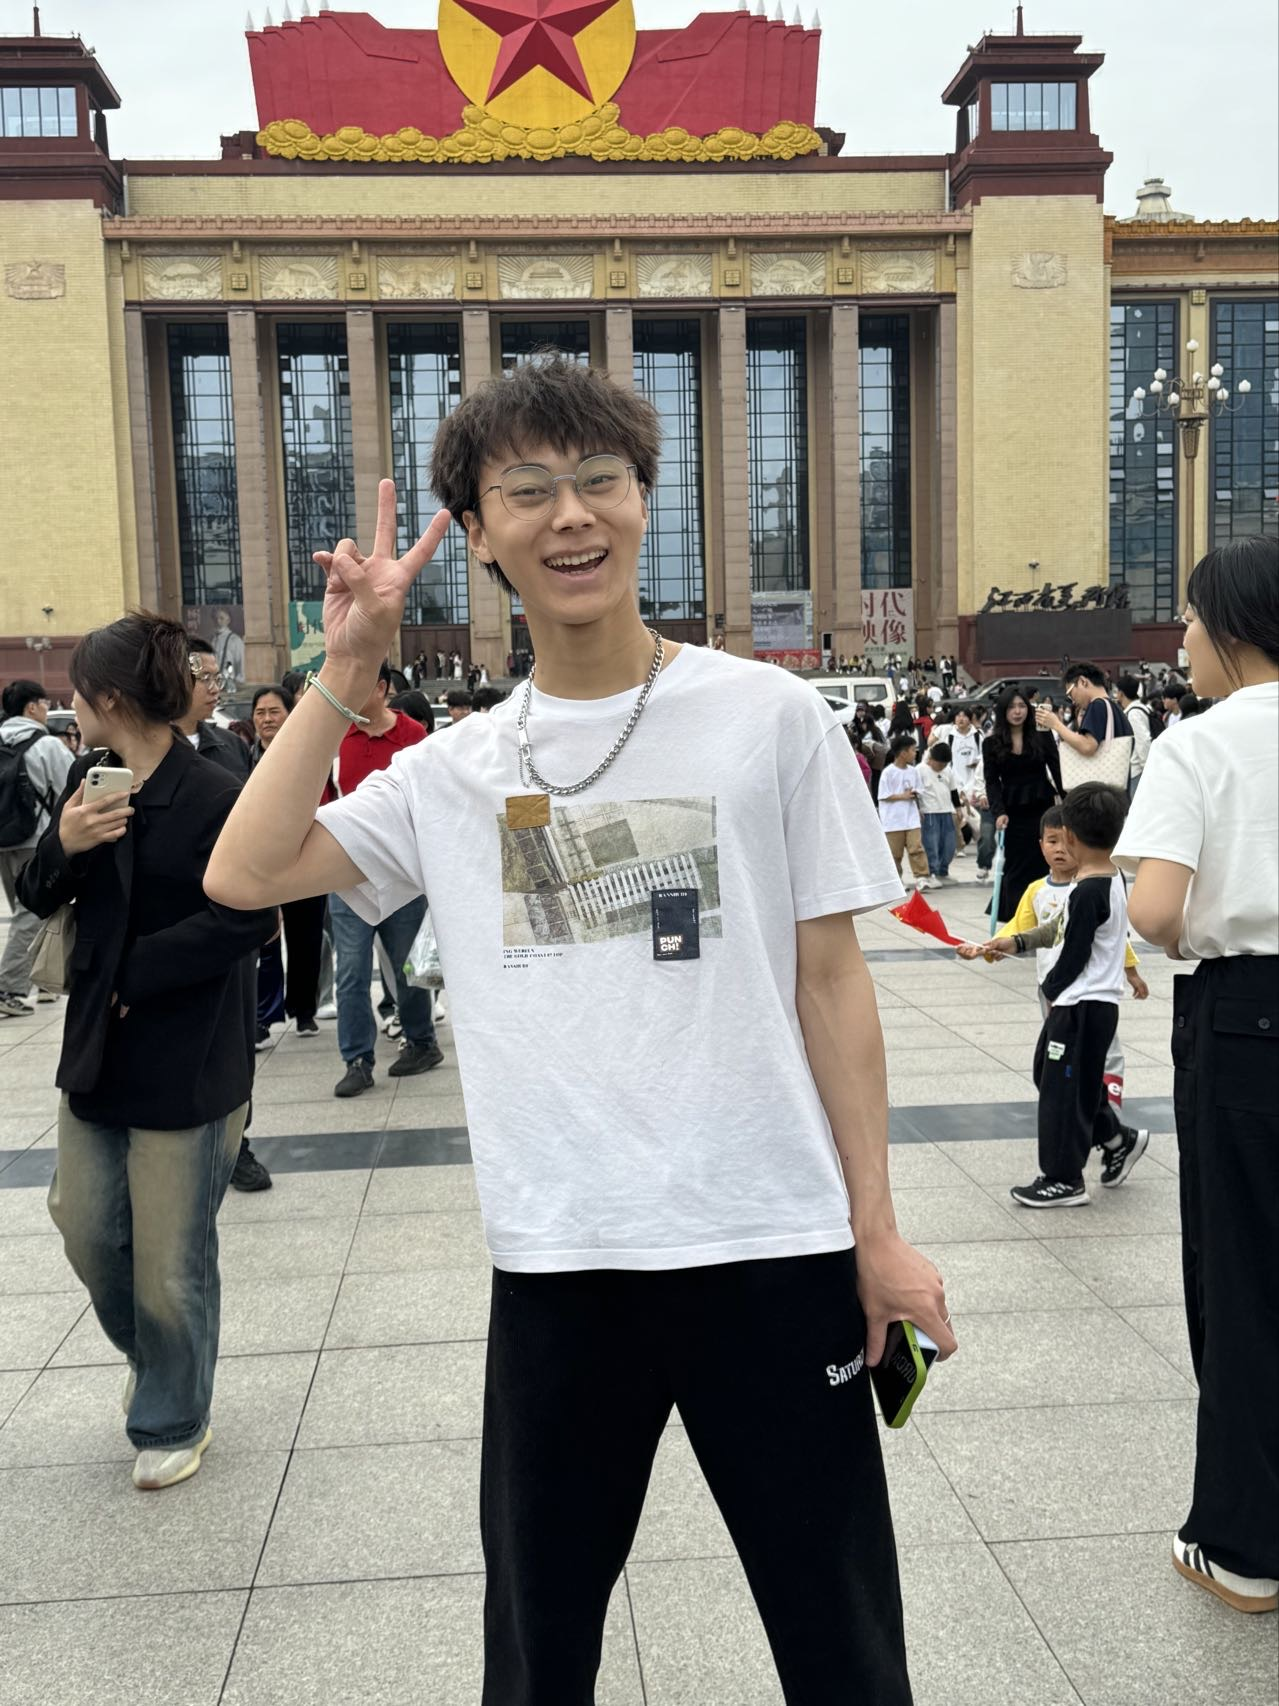
\includegraphics[width=0.5\textwidth]{figures/articles/02-8.jpg}
        \caption*{\small{2024年5月1日于八一广场}}
    \end{figure}

    \bottomtext{“匆忙的脚步里，也藏着温柔的瞬间。”}

\end{spacing}

\clearpage